\documentclass{article}



\usepackage{arxiv}

\usepackage[utf8]{inputenc} % allow utf-8 input
\usepackage[T1]{fontenc}    % use 8-bit T1 fonts
\usepackage{hyperref}       % hyperlinks
\usepackage{url}            % simple URL typesetting
\usepackage{booktabs}       % professional-quality tables
\usepackage{amsfonts}       % blackboard math symbols
\usepackage{nicefrac}       % compact symbols for 1/2, etc.
\usepackage{microtype}      % microtypography
\usepackage{graphicx}
\usepackage{natbib}
\usepackage{doi}
\newcommand{\theHalgorithm}{\arabic{algorithm}}
\usepackage{float}
\usepackage{tikz}
\usepackage{url}

\usepackage{booktabs}  
\usepackage{subcaption}
\usepackage{amsmath}
\usepackage{amssymb}
\usepackage{amsthm}

\theoremstyle{plain}
\newtheorem{theorem}{Theorem}[section]
\newtheorem{conjecture}{Conjecture}[section]
\newtheorem{proposition}[theorem]{Proposition}
\newtheorem{lemma}[theorem]{Lemma}
\newtheorem{corollary}[theorem]{Corollary}
\theoremstyle{definition}
\newtheorem{definition}[theorem]{Definition}
\newtheorem{assumption}[theorem]{Assumption}
\theoremstyle{remark}
\newtheorem{remark}[theorem]{Remark}


\title{Are GNNs doomed by the topology of their input graph?}

%\date{September 9, 1985}	% Here you can change the date presented in the paper title
%\date{} 					% Or removing it

\author{Amine Mohamed Aboussalah \\ NYU Tandon School of Engineering \\ \texttt{ama10288@nyu.edu} \\
    \And
    Abdessalam Ed-dib \\
    NYU Tandon School of Engineering \\
    \texttt{ae2842@nyu.edu}
}


\makeatletter
\def\blfootnote{\xdef\@thefnmark{}\@footnotetext}
\makeatother
% Uncomment to remove the date
%\date{}

% Uncomment to override  the `A preprint' in the header
\renewcommand{\headeright}{Under review -- 
 ICML2025}
%\renewcommand{\undertitle}{Technical Report}
\renewcommand{\shorttitle}{Are GNNs doomed by the topology of their input graph?}

%%% Add PDF metadata to help others organize their library
%%% Once the PDF is generated, you can check the metadata with
%%% $ pdfinfo template.pdf
\hypersetup{
pdftitle={Are GNNs doomed by the topology of their input graph?},
pdfsubject={cs.AI, cs.LG, stat.ML, math.GT},
pdfauthor={Amine M. Aboussalah, Abdessalam Ed-dib,},
pdfkeywords={Information Geometry, Graph Neural Networks, Oversmoothing},
}

\begin{document}

\maketitle

\begin{abstract}
Retrieval-Augmented Generation (RAG) is often used with Large Language Models (LLMs) to infuse domain knowledge or user-specific information. In RAG, given a user query, a retriever extracts chunks of relevant text from a knowledge base. These chunks are sent to an LLM as part of the input prompt. Typically, any given chunk is repeatedly retrieved across user questions. However, currently, for every question, attention-layers in LLMs fully compute the key values (KVs) repeatedly for the input chunks, as state-of-the-art methods cannot reuse KV-caches when chunks appear at arbitrary locations with arbitrary contexts. Naive reuse leads to output quality degradation.  This leads to potentially redundant computations on expensive GPUs and increases latency. In this work, we propose \sys, a system for managing and reusing precomputed KVs corresponding to the text chunks (we call \textit{chunk-caches}) in RAG-based systems. We present how to identify \hl{\textit{chunk-caches} that are reusable}, how to efficiently perform a small fraction of recomputation to \textit{fix} the cache to maintain output quality, and how to efficiently store and evict \textit{chunk-caches} in the hardware for maximizing reuse while masking any overheads. With real production workloads as well as synthetic datasets, we show that \sys reduces redundant computation by \textbf{51\%} over SOTA prefix-caching and \textbf{75\%} over full recomputation.
\hl{Additionally, with continuous batching on a real production workload, we get a \textbf{1.6$\times$} speedup in throughput and a \textbf{2$\times$} reduction in end-to-end response latency over prefix-caching while maintaining quality, for both the \llama-3-8B and \llama-3-70B models. 
}
\end{abstract}






% keywords can be removed
\keywords{Graph Neural Networks \and $k$-hop Similarity  \and Oversmoothing}


\documentclass[../main.tex]{subfiles}
\graphicspath{{../images/}}
\makeatletter
\def\input@path{{../images/}}
\makeatother
\begin{document}
\section{Introduction}
\begin{figure}
\centering
\begin{tikzpicture}
\node[inner sep=0pt] (ws) at (0, 0) {
\includegraphics[height=.4\textwidth, trim={10cm 0 10cm 0},clip]{world_space.png}};
\node[inner sep=0pt] (cs) at (6,0) {\includegraphics[height=.4\textwidth, trim={10cm 1cm 10cm 4cm},clip]{conf_space.png}};
\end{tikzpicture}
\vspace{-5pt}
\label{fig:pbrm_intro}
\caption{\textbf{Left}: Shows world space obstacles as grey spheres. Robots start and goal configuration is colored red and green, respectively. Configurations along the computed path are colored transparent blue. \textbf{Right:} Mapped world space scenario to configuration space. Obstacle region is the grey mesh. Red spheres are collision-free regions computed by the neural SCDF. The optimized shortest path in the convex corridor is the blue curve.}
\vspace{-25pt}
\end{figure}
Motion planning is the problem of finding a collision-free trajectory that connects a given start and goal configuration. The planning takes place in the configuration space of the robot. For single body robots, like mobile robots or drones, the configuration space and the world space are usually the same. This simplifies the planning, since explicit obstacle representations are available which enables geometrical tools like separating hyperplanes, smallest distance to obstacles etc., to be used when designing motion planning algorithms. For multi-body robots like manipulators, the situation is completely different. The world space obstacles are usually mapped to non-convex regions, and to make the problem even harder, the mapping is usually not known. Forming explicit representations of the obstacle region in the configuration space is usually too expensive or intractable. Despite all of this, sampling based planners are used with great success, which mainly is due to their use of implicit representations of the obstacle region. The basic idea is to construct a graph in the configuration space that covers and connects the collision-free region. From this graph, a path can be extracted that connects a given start and goal configuration. The approach is computationally expensive, since the graph is constructed with the smallest geometrical building block available, points, which represents a collision-check. Furthermore, the extracted paths from the graph are non-smooth and jagged due to the stochastic nature of the approach. This adds an additional post-processing step to the process, where the paths are shortcutted and smoothened, before the path can be used for tracking. Clearly a lot of time is invested to form this graph and produce smooth paths. Thus, if the obstacles start to move, then all of this work is done in no use, since all points that make up this graph need to be re-verified, which is simply too time consuming to be done in real time.
\\\\
In this work, we want to address the existing drawbacks of the sampling based planners. Our main contribution is an improved motion planner where each vertex in the graph covers a collision-free region in the form of a sphere instead of a point and where the edges are formed with neighboring intersecting spheres. This representation has the advantage of instead of returning piecewise linear paths, returning a sequence of overlapping spheres, i.e. a convex corridor, that connects a given start and goal configuration, illustrated in Figure \ref{fig:pbrm_intro}. This convex corridor allows us to use convex optimization to produce smooth trajectories, instead of computationally expensive post-processing methods. The representation further allows us to estimate the coverage of the collision-free space, which gives us awareness and feedback in the offline roadmap construction phase. Finally, our representation is simple to adapt to moving obstacles, simply requery for the new radii and recheck for intersections. 
\\\\
The spherical collision-free regions are formed using a signed distance function (SDF), which is a function that returns the smallest distance from an arbitrary point to the boundary of an obstacle. As the name implies, the distance is signed, thus if the point is inside the obstacle it is negative otherwise positive. If the distance is positive, a sphere with radius equal to the distance is guaranteed to cover a collision-free region. Using an SDF in motion planning is not new, but what is novel about our approach is that we express the distance in the configuration space instead of the world space and by doing so allows us to form these convex collision-free regions. We refer to the resulting SDF as a signed configuration distance function (SCDF). Computing an SCDF analytically is non-trivial, our approach is therefore to parameterize the SCDF with a deep neural network and learn the mapping by supervised learning. Our resulting neural SCDF can compute distances for different parameter values of obstacle shapes and we also show how multiple distances can be combined, thus making our approach flexible.
\section{Related work}
Motion planning algorithms can roughly be divided into three families, grid-based, sampling based and optimization based methods. Grid-based methods (GBM) discretize the planning space from which a graph is then compiled. A standard search method is A$^\star$ \citep{a_star}, which is classified as an \textit{informed} search method, since it employs a heuristic function to speed up the search. A$^\star$ guarantees to return an optimal path at the level of discretization used. GBMs usually discretize the planning space by a regular lattice and this limits the GBMs to problems with low dimensionality due to the curse of dimensionality. Thus, GBMs are usually limited to single-body robots where the degrees of freedom (DOF) are low. To overcome the inherent scaling problem with the GBMs, stochastic methods are usually used for multi-body robots. These methods are termed as sampling-based methods (SBM) and core members within this family are the rapidly-exploring random trees (RRT) \citep{rrt} and the probabilistic roadmap (PRM) \citep{prm}. RRT grows a tree from the start configuration and explores the collision-free region in a rapid way until it is able to connect to the goal region. RRT is usually improved by bi-directional planning \citep{rrt_connect}, i.e. an additional tree is grown from the goal configuration and the trees are tested for connection after any tree has been expanded. RRT is a single-query method, thus it searches for a path from scratch each time it is queried. Contrary to this, PRM is a multi-query method, which solves for multiple queries without starting from scratch. PRM does this by creating a roadmap (graph) that covers the collision-free space as an offline step. The graph is then used to solve for multiple queries. PRMs are used in cases where the environment does not change since the extra offline step is too computationally costly and needs to be re-done if the environment is changed. In our work, we address this inherent issue by using a different roadmap representation. Our vertices in the graph cover a collision-free region in the form of spheres and we form the edges by checking for intersecting spheres. If something in the environment changes, we recompute the spheres radii and recheck the intersections, without relying on collision detection. We use a trained neural network to compute the sphere radius, therefore querying for the radius can be done fast, hence our representation enables the PRM for dynamic environments.
\\\\
In the recent decades, optimization based methods (OBM) \citep{chomp, schulman, itomp, stomp} have been introduced as an alternative to SBM for multi-body robots. Like the SBM, the OBMs scale well to higher dimensional problems and produce smoother motion. It is common to use a SDF in the optimization since it is a smooth function, thus enabling gradient-based methods. However, the standard way of expressing the SDF is in world space. The distance therefore needs to be mapped to the configuration space by the forward kinematics. This mapping makes the optimization problem a non-linear program (NLP), which is computationally expensive to solve. Recently, a different approach has been proposed. In \cite{mp_gcs} motion planning is formulated as a convex optimization problem by using the graph of convex sets framework \citep{gcs}. The underlying idea is to decompose the collision-free space into intersecting convex sets from which a convex optimization problem is formulated. In cases where an explicit representation of the obstacles in the configuration space exists, like for single-body robots, creating collision-free convex regions can be done fast \citep{iris}. For multi-body robots, this is non-trivial. Existing work does this successfully \citep{iris_nlp, iris_c} by an optimization based approach, but the methods are still too time consuming to be used in the presence of moving obstacles. Our approach is instead to use deep learning to learn an SDF expressed in the configuration space. With this, we can query for shortest distances to the collision boundary, which allows us to expand spherical regions which are collision-free. Our approach is fast and therefore enables our suggested roadmap planner to be used in dynamic environments.
\\\\
Recent research has focused on learning collision detection \citep{fk_kernel_distance, diffco, graphdistnet} by predicting the signed distance between the robot links and the surrounding obstacles in the world space. The learned SDF is used in trajectory optimization but since the distance is expressed in the world space, the problem becomes an NLP and therefore takes a long time to solve. We take a novel approach and suggest to instead express the signed distance in the configuration space. This allows us to improve the PRM at the same time as it enables convex optimization for trajectory optimization, which runs faster and is more reliable than NLP solvers. In \cite{cspf} a learned signed distance function in the configuration space is proposed similar to our approach. However, their approach is restricted to point cloud representations, while we propose to represent the obstacles as parameterized geometric shapes, e.g. spheres. Furthermore, we also show how to use our learned SCDF to improve an existing roadmap planner.
\section{Problem formulation}
A robot is located in the world space, $\W \subset \R^3 $. The unique location of the robot is given by its configuration $\q \in \C$, where $\C$ is the configuration space. The set of points covered by the robots bodies at a certain configuration is expressed as $\B(\q) \subset \W$. The robot is surrounded by $\NrObst$ obstacles $\O = \bigcup_{i=1}^{\NrObst} \O_i$, where  $\O_i \subset \W$. The representation of the obstacle in the configuration space is the set $\C\O_i = \{\q \in \C \: |\: \B(\q) \cap \O_i \neq \emptyset \}$. The obstacle space is formed as $\Co = \bigcup_{i=1}^{\NrObst} \C \O_i$. The complement is referred to as the free space, $\Cf = \C \setminus \Co$. The path planning problem is a tuple, ($\Cf$, $\qStart$, $\qGoal$), where we want to connect a query pair, consisting of a start, $\qStart$, and goal configuration, $\qGoal$, with a geometric path, $\q(s): [0, 1] \mapsto \Cf$, such that $\q(0)=\qStart$ and $\q(1)=\qGoal$, or report correctly when such a path does not exist.
\end{document}


\section{Preliminaries}\label{sec:preliminaries}



%We denote by $(\Ac(x_\Ac),\Bc(x_\Bc))(z)$ a random execution of $\pi$ with private inputs $(x_\Ac,y_\Ac)$, and common input $z$.

%\Jnote{Move to DP}
% At the end of such an execution, the protocol outputs a public transcript denoted by the random variable $\trans_\pi(x_\Ac,x_\Ac,z)$ we denotes the common as $\out(\trans_\pi(x_\Ac,x_\Ac,z)$, and each party $\Pc \in \set{\Ac,\Bc}$ obtains his view denoted $\view^\Pc_\pi(x_\Ac,x_\Bc,z)$, which may also contain a ``local output'' \Jnote{Local} $\out^\Pc(x_\Ac,x_\Bc,z)$ (if the protocol specifies such an output). \Jnote{Common output, and parties output}


\subsection{Distributions and Random Variables}\label{sec:prelim:dist}
The support of a distribution $P$ over a finite set $\cS$ is defined by $\Supp(P) \eqdef \set{x\in \cS: P(x)>0}$. For a distribution or a random variable $D$, let $d\from D$ denote that $d$ was sampled according to $D$. Similarly,  for a set $\cS$, let $x \from \cS$ denote that $x$ is drawn uniformly from $\cS$, and denote by $\cU_{\cS}$ the uniform distribution over $\cS$. For a finite set $\cX$ and a distribution $C_X$ over $\cX$, we use the capital letter $X$ to denote the random variable that takes values in $\cX$ and is sampled according to $C_X$. The {\sf statistical distance} (\aka {\sf~variation distance}) of two distributions $P$ and $Q$ over a discrete domain $\cX$ is defined by $\sdist{P}{Q} \eqdef \max_{\cS\subseteq \cX} \size{P(\cS)-Q(\cS)} = \frac{1}{2} \sum_{x \in \cS}\size{P(x)-Q(x)}$. 
For a vector $x = (x_1,\ldots,x_n)$ and index $i\in [n]$, we let $x_{-i} = (x_1,\ldots,x_{i-1},x_{i+1},\ldots,x_n)$ and $x^{(i)} = (x_1,\ldots,x_{i-1}, -x_i, x_{i+1},\ldots,x_n)$, for a set $\cS \subseteq [n]$ we let $x_{\cS} = (x_i)_{i \in \cS}$ and $x_{-\cS} = (x_i)_{i \in [n]\setminus \cS}$, and for a vector $r \in \zo^n$ we let $x_r = (x_i)_{\set{i \colon r_i = 1}}$ and $x_{-r} = (x_i)_{\set{i \colon r_i = 0}}$.

%For $n \in \N$ we let $U_n$ be the uniform distribution over $\oo^n$, and let $S_n$ be the distribution induces by the sum of $n$ i.i.d.\ random variables, each is distributed according to $U_1$. Let $\cN(0,1)$ be the standard normal distribution.
%For a distribution $\cD$ and a function $f$, we define by $f(\cD)$ the distribution that is induced by the output of $f(x)$ for $x \from \cD$. 





% \begin{theorem}[\cite{McGregorMPRTV10}]\label{thm:sv-extracotr}
% 	\Enote{Remove if not needed}
% 	There is a constant $c$ to make the following holds. Let $X$ be an $\alpha$-SV source on $\{0,1\}^n$, let $Y$ be a source on $\{0,1\}^n$ with min-entropy at least $\beta n$ (independent from $X$), and let $Z=\ip{X,Y}\mbox{mod m}$ for some $m\in\mathbb{N}$. Then for every $\delta\in[0,1]$, the random variable $(Y,Z)$ is $\delta$-close to $(Y,U)$ where $U$ is uniform on $\mathbb{Z}_m$ and independent of $Y$, provided that
% 	$$
% 	n\geq c\cdot\frac{m^2}{\alpha\beta}\cdot\log(\frac{m}{\beta})\cdot\log(\frac{m}{\delta}).
% 	$$
% \end{theorem}



\Enote{I removed the definition of DP since it already appears in the intro}
\remove{
\subsection{Differential Privacy}\label{sec:prelim:DP}
We use the following standard definition of (information theoretic) differential privacy, due to \citet{DMNS06}. For notational convenience, we focus on databases over $\oo$.
\begin{definition}[Differentially private mechanisms]\label{def:mech}
	A randomized function $f\colon\oo^n\mapsto \zs$ is an {\sf $n$-size, $(\eps,\delta)$-differentially private mechanism} (denoted $(\eps,\delta)$-\DP) if for every neighboring $w,w'\in \oo^n$ and every function $g\colon \zs\mapsto \zo$, it holds that 
	$$
	\pr{g(f(w))=1}\leq e^{\eps}\cdot \pr{g(f(w'))=1} +\delta.
	$$ 	
	If $\delta=0$, we omit it from the notation.
\end{definition}
}


\subsubsection{Computational Differential Privacy}
There are several ways for defining computational differential privacy (see \cref{sec:related-works}). We use the most relaxed version due to \cite{BNO08}. For notational convenience, we focus on databases over $\oo$.
\begin{definition}[Computational differentially private mechanisms]\label{def:ComMech}
	A randomized function ensemble $f=\set{f_\pk\colon\oo^{n(\pk)}\mapsto \zs}$ is an {\sf $n$-size, $(\eps,\delta)$-computationally differentially private} (denoted $(\eps,\delta)$-$\CDP$) if for every poly-size circuit family $\set{\Ac_\pk}_{\pk\in \N}$, the following holds for every large enough $\pk$ and every neighboring $w,w'\in\oo^{n(\pk)}$:
	$$
	\pr{\Ac_\pk(f_\pk(w))=1}\leq e^{\eps(\pk)}\cdot \pr{\Ac_\pk(f_\pk(w'))=1} +\delta(\pk).
	$$ 
	If $\delta(\pk) = \negl(\pk)$, we omit it from the notation. 
\end{definition}



\subsubsection{Two-Party Differential Privacy}\label{sec:DP}
In this section we formally define distributed differential privacy mechanism (\ie protocols). %For the ease of notation, we consider protocol with no common input.

\begin{definition}\label{def:DP}%\Nnote{fix security parameter}
	A two-party protocol $\Pi=(\Ac,\Bc)$ is {\sf $(\eps,\delta)$-differentially private}, denoted $(\eps,\delta)$-$\DP$, if the following holds for every algorithm $\Dc$: let $\V^\Pc(x,y)(\pk)$ be the view of party $\Pc$ in a random execution of $\Pi(x,y)(1^\pk)$. Then for every $\pk,n \in \N$, $x\in \oo^n$ and neighboring $y,y'\in\oo^n$:
	\begin{align*}
	\pr{\Dc(V^\Ac(x,y)(\pk))=1}\le e^{\eps(\pk)}\cdot \pr{\Dc(V^\Ac (x,y')(\pk))=1}+\delta(\pk),
	\end{align*} 
	and for every $y\in \oo^n$ and neighboring $x,x'\in\oo^{n}$:
	\begin{align*}
	\pr{\Dc(V^\Bc(x,y)(\pk))=1}\le e^{\eps(\pk)}\cdot \pr{\Dc(V^\Bc (x',y)(\pk))=1}+\delta(\pk).
	\end{align*} 	
	Protocol $\Pi$ is {\sf $(\eps,\delta)$-computational differentially private}, denoted $(\eps,\delta)$-$\CDP$, if the above inequalities only hold for a non-uniform \ppt $\Dc$ and large enough $\pk$. We omit $\delta = \negl(\pk)$ from the notation. \footnote{Note that define we give for two-party differentially private protocols is a semi-honest definition, in which we ask for the security to hold when the parties interact in an honest execution of the protocol. Since we are proving a lower bound, starting from this weaker guarantee (as opposed to security against malicious players), yields a stronger result.}
\end{definition}
%We omit $\delta$ from the notation if $\delta$ is a negligible function of $n$.

%\Enote{simulation-based}
\begin{remark}[The definition for computational differential privacy we use]\label{rem:comDPChannel} 
	An alternative, stronger definition of computational differential privacy, known as simulation-based computational differential privacy, requires that the distribution of each party’s view be computationally indistinguishable from a distribution that ensures privacy in an information-theoretic sense. \cref{def:DP} is a weaker notion in comparison. Consequently, establishing a lower bound for a protocol that satisfies this weaker guarantee (as we do in this work) yields a stronger result.%Actually, our lower bound only requires the privacy to hold against \emph{uniform} external observer.
	%\Nnote{Maybe add: When only interesting in \Dp against external observer, the two definitions can be achieve using key-agreement and (single-party) \Dp mechanism. }
\end{remark}




\subsection{Useful Claims}
\remove{
In this section, we state generic lemmas and propositions that we will use later in our proofs.

The following lemma which we prove in \cref{sec:missing-proofs:distance-I}, measures the distance between two uniform stings conditioned one a random index $i$ either being fixed to $0$ or to $1$.

\def\distanceILemma{
    Let $R \la \zo^n$. For any (randomized) function $f:\{0,1\}^n\rightarrow \{0,1\}$ and $\alpha > 0$, it holds that
    \begin{align}\label{eq:f-alpha}
        \ppr{i \la [n]}{\size{\:\ex{f(R) \mid R_i = 0}-\ex{f(R) \mid R_i = 1}\:}\geq \alpha} \leq \frac{2}{n \alpha^2},
    \end{align}
    where the expectations are taken over $R$ and the randomness of $f$.
}

\begin{lemma}\label{lem:distance-I}
    \distanceILemma
\end{lemma}
}

The following two propositions state that given the output of a differentially private function, it is not possible to predict well even a random index (even if all other indexes are leaked). The first proposition handles the information-theoretic case and the second handles the computation case. Both propositions are proven in \cref{sec:missing-proofs:hard-to-guess}. 

\def\propHardToGuessInf{
    Let $f\colon \oo^n \rightarrow \cY$ be an $(\eps,\delta)$-\DP function, let $g \colon [n] \times \oo^{n-1} \times \cY \rightarrow \set{-1,1,\bot}$ be a (randomized) function, and let $X = (X_1,\ldots,X_n) \la \oo^n$. Then the following holds for every $i \in [n]$ where $X_i^* = g(i,X_{-i},f(X_1,\ldots,X_n))$:
    \begin{align*}
        \pr{X_i^* = X_i} \leq e^{\eps}\cdot \pr{X_i^* = -X_i} + \delta.
    \end{align*}
}

\begin{proposition}\label{prop:hard-to-guess-inf}
    \propHardToGuessInf
\end{proposition}


\def\propHardToGuessComp{
    Let $f = \set{f_{\pk} \colon \oo^{n(\pk)} \rightarrow \zo^{m(\pk)}}_{\pk \in \bbN}$ be an $(\eps,\delta)$-\CDP function ensemble, and let $\set{g_{\pk}}_{\pk \in \bbN}$ be a poly-size circuit family. Then, for large enough $\pk$ and $X = (X_1,\ldots,X_{n(\pk)}) \la \oo^{n(\pk)}$, the following holds for every $i \in [n(\pk)]$ where $X_i^* = g_{\pk}(i,X_{-i},f_{\pk}(X_1,\ldots,X_n))$:
    \begin{align*}
        \pr{X_i^* = X_i} \leq e^{\eps(\pk)}\cdot \pr{X_i^* = -X_i} + \delta(\pk).
    \end{align*}
}

\begin{proposition}\label{prop:hard-to-guess-comp}
    \propHardToGuessComp
\end{proposition}





\remove{
\Enote{Chao's old statement:}
\begin{lemma}\label{lem:distance-I-old}
        Let $R \la \zo^n$. 
	For any function $f:\{0,1\}^n\rightarrow \{0,1\}$ and $\alpha<0.01$, it holds that
	$$
	\Pr_{i\la[n]}\left[\: \size{\:\mathbb{E}[f(R) \mid R_i = 0]-\mathbb{E}[f(R) \mid R_i = 1]\:}\geq \alpha\right]\leq \frac{2+2\log(\frac{1}{\alpha})}{n\alpha^2}.
	$$
\end{lemma}
\begin{proof}
	Define $S_1=\{r \in \zo^n \colon f(r)=1\}$. Then for any $i\in[n]$, we have
	$$
	\begin{array}{rl}
		\size{\mathbb{E}[f(R) \mid R_i = 0]-\mathbb{E}[f(R) \mid R_i = 1]}
		&=\size{\Pr[R\in S_1|R_i=0]-\Pr[R\in S_1|R_i=1]}\\
		&=\size{\frac{\Pr[R_i=0|R\in S_1]\cdot\Pr[R\in S_1]}{\Pr[R_i=0]}-\frac{\Pr[R_i=1|R\in S_1]\cdot\Pr[R\in S_1]}{\Pr[R_i=1]}}\\
		&=\frac{2\size{S_1}}{2^n}\size{\Pr[R_i=0|R\in S_1]-\Pr[R_i=1|R\in S_1]}
	\end{array}
	$$
	When $|S_1|\leq \alpha\cdot 2^{n-1}$, we have $\size{\mathbb{E}[f(R) \mid R_i = 0]-\mathbb{E}[f(R) \mid R_i = 1]}\leq\frac{2\size{S_1}}{2^n}\leq \alpha$ for any $i\in[n]$. Hence, in the following, we assume $|S_1|> \alpha\cdot 2^{n-1}$.

	%Define $I_{bad}=\{i|\size{\Pr[R_i=0|R\in S_1]-\Pr[R_i=1|R\in S_1]}>2\alpha\}$ and $k=\size{I_{bad}}$, then for any $i\notin I_{bad}$, we have 
    %$$
    %\begin{array}{rl}
    %    2\alpha&\geq \size{\Pr[R_i=0|R\in S_1]-\Pr[R_i=1|R\in S_1]}\\
    %    &=\size{\frac{\Pr[R\in S_1|R_i=0]\cdot\Pr[R_i=0]}{\Pr[R\in S_1]}-\frac{\Pr[R\in S_1|R_i=1]\cdot\Pr[R_i=1]}{\Pr[R\in S_1]}}\\
    %    &=\size{\Pr[R\in S_1|R_i=0]-\Pr[R\in S_1|R_i=1]}\cdot\frac{1}{2\Pr[R\in S_1]}\\
    %    &\geq \size{\mathbb{E}[f(R) \mid R_i = 0]-\mathbb{E}[f(R) \mid R_i = 1]}\cdot \frac{1}{2},
    %\end{array}
    %$$ 
    %where the last inequality is because $\Pr[R\in S_1]\leq 1$. So that $\size{\mathbb{E}}[f(R) \mid R_i = 0]-\mathbb{E}[f(R) \mid R_i = 1]\leq %4\alpha$.
    Define $I_{bad}=\{i \colon \size{\Pr[R_i=0|R\in S_1]-\Pr[R_i=1|R\in S_1]} \geq 2\alpha\}$ and $k=\size{I_{bad}}$, and denote $I_{bad}=\{i_1,\dots,i_k\}$. Define $(X_{i_1}, \ldots X_{i_k}) = (R_{i_1},\dots,R_{i_k})\mid_{R \in S_1}$. 
    Consider the min-entropy
	$$
	\begin{array}{rl}
		H_{min}(X_{i_1},\dots,X_{i_k})&\leq H(X_{i_1},\dots,X_{i_k})\\
		&\leq \sum_{j=1}^k H(X_{i_j})\\
		&\leq k\cdot \left(-(\frac{1}{2}+2\alpha)\cdot\log(\frac{1}{2}+2\alpha)-(\frac{1}{2}-2\alpha)\cdot\log(\frac{1}{2}-2\alpha)\right)\\
            &=k\cdot \left(-(\frac{1}{2}+2\alpha)\cdot(\log(1+4\alpha)-1)-(\frac{1}{2}-2\alpha)\cdot(\log(1-4\alpha)-1)\right)\\
            &=k\cdot \left(1-(\frac{1}{2}+2\alpha)\cdot\log(1+4\alpha)-(\frac{1}{2}-2\alpha)\cdot\log(1-4\alpha)\right),
		
	\end{array}
	$$
	where $H_{min}(Y)$ is the minimum entropy of $Y$ and $H(Y)$ is the Shannon entropy of $Y$.\Enote{add to preliminaries.}
        The third inequality holds since by the definition of $I_{bad}$, for every $j \in [k]$ it holds that $\size{\pr{X_{i_j} = 1}-\pr{X_{i_j} = 0}} > 2\alpha$, and therefore $H(X_{i_j}) \leq H(1/2 + 2\alpha)$\Enote{define}.
	
	Therefore, there exists $b_1,\dots,b_k\in\{0,1\}$, such that 
	
	\begin{align}\label{eq:min-entropy-result}
		\Pr\left[(R_{i_1},\ldots,R_{i_k}) = (b_1,\ldots,b_k) \mid R\in S_1\right]
		&= \pr{(X_{i_1},\ldots,X_{i_k}) = (b_1,\ldots,b_k)}\\
		&= 2^{-H_{min}(X_{i_1},\dots,X_{i_k})}\nonumber\\
		&\geq 2^{k\cdot \left(-1+(\frac{1}{2}+2\alpha)\cdot\log(1+4\alpha)+(\frac{1}{2}-2\alpha)\cdot\log(1-4\alpha)\right)}.\nonumber
	\end{align}
	
	Let $S_{bad}=\{r \in \zo^n  \colon \set{(r_{i_1},\ldots,r_{i_k}) = (b_1,\ldots,b_k)} \land \set{r\in S_1}\}$.
	It holds that
	\begin{align*}
		|S_{bad}|
		&= \size{S_1} \cdot \Pr\left[(R_{i_1},\ldots,R_{i_k}) = (b_1,\ldots,b_k) \mid R\in S_1\right]\\
		&\geq \alpha\cdot 2^{n-1}\cdot2^{k\cdot \left(-1+(\frac{1}{2}+2\alpha)\cdot\log(1+4\alpha)+(\frac{1}{2}-2\alpha)\cdot\log(1-4\alpha)\right)},
	\end{align*} 
	where the inequality holds by \cref{eq:min-entropy-result} and since $\size{S_1} \geq \alpha\cdot 2^{n-1}$.
	Notice that any string in $S_{bad}$ depends on at most $n-k$ bits. It implies that $|S_{bad}|\leq 2^{n-k}$. Therefore, we have
	$$
	\begin{array}{rl}
		&2^{n-k}\geq \alpha\cdot 2^{n-1}\cdot2^{k\cdot \left(-1+(\frac{1}{2}+2\alpha)\cdot\log(1+4\alpha)+(\frac{1}{2}-2\alpha)\cdot\log(1-4\alpha)\right)} \\
		\Rightarrow& n-k \geq \log \alpha+n-1+k\cdot \left(-1+(\frac{1}{2}+2\alpha)\cdot\log(1+4\alpha)+(\frac{1}{2}-2\alpha)\cdot\log(1-4\alpha)\right)\\
		\Rightarrow& 1-\log \alpha \geq k\cdot((\frac{1}{2}+2\alpha)\cdot\log(1+4\alpha)+(\frac{1}{2}-2\alpha)\cdot\log(1-4\alpha))\\
		\Rightarrow& 1-\log \alpha \geq k\cdot(4\alpha\cdot\log(1+4\alpha)+(\frac{1}{2}-2\alpha)\cdot\log(1-16\alpha^2))\\
        \Rightarrow& 1-\log\alpha \geq k\cdot(15.9\alpha^2-8\alpha^2+32\alpha^3)=k\cdot(7.9\alpha^2+32\alpha^3)>0.5k\alpha^2\\
		\Rightarrow& k\leq \frac{2-2\log \alpha}{\alpha^2} = \frac{2+2\log (1/\alpha)}{\alpha^2},
	\end{array}
	$$
	Where the third transition holds since 
	\begin{align*}
		\lefteqn{(\frac{1}{2}+2\alpha)\cdot\log(1+4\alpha)+(\frac{1}{2}-2\alpha)\cdot\log(1-4\alpha)}\\
		&= 4\alpha\cdot\log(1+4\alpha) + (\frac{1}{2}-2\alpha)\paren{\log(1+4\alpha)+\log(1-4\alpha)}\\
		&= 4\alpha\cdot\log(1+4\alpha)+(\frac{1}{2}-2\alpha)\cdot\log(1-16\alpha^2),
	\end{align*}
	and the forth transition holds since $4\alpha\cdot\log(1+4\alpha)+(\frac{1}{2}-2\alpha)\cdot\log(1-16\alpha^2) > 15.9\alpha^2-8\alpha^2+32\alpha^3$ for $\alpha < 0.01$.
	Thus, we conclude that 
	$$
	\Pr_{i\la[n]}\left[\size{\mathbb{E}[f(R) \mid R_i=0]-\mathbb{E}[f(R) \mid R_i = 1]}\geq \alpha\right]\leq \frac{k}{n}\leq \frac{2+2\log (1/\alpha)}{n\alpha^2}.
	$$
\end{proof}
}


\subsection{Channels and Two-Party Protocols}\label{sec:protocol}

\paragraph{Channels.}A channel is simply a distribution of a pair of tuples defined as follows. 
\begin{definition}[Channels]\label{def:channel} A {\sf channel} $C_{(X,U)(Y,V)}$ of size $\isize$ over alphabet $\Sigma$ is a probability distribution over $(\Sigma^\isize \times\zo^\ast) \times(\Sigma^\isize \times\zo^\ast)$. The ensemble $C_{(X,U)(Y,V)}= \set{C_{(X_\pk,U_\pk)(Y_\pk,V_\pk)}}_{\pk\in \N}$ is an $\isize$-size channel ensemble, if for every $\pk\in \N$, $C_{(X_\pk,U_\pk)(Y_\pk,V_\pk)}$ is an $\isize(\pk)$-size channel. %We denote a channel of size one by a \emph{single-bit} channel. 
We refer to $X$ and $Y$ as the {\sf local outputs}, and to $U$ and $V$ as the {\sf views}.	
\end{definition}

We view a  channel as the experiment in which there are two parties $\Ac$ and $\Bc$.  Party $\Ac$ receives ``output'' $X$ and ``view'' $U$, and party $\Bc$ receives ``output'' $Y$ and ``view'' $V$. Unless stated otherwise, the channels we consider are over the alphabet $\Sigma = \oo$. We naturally identify channels with the distribution that characterizes their output.








\subsubsection{Two-Party Protocols}

A two-party protocol $\Pi=(\Ac,\Bc)$ is \ppt if the running time of both parties is polynomial in their input length. We let $\Pi(x,y)(z)$ or $(\Ac(x),\Bc(y))(z)$ denote a random execution of $\Pi$ on a common input $z$, and private inputs $x,y$.%We assume \wlg that a protocol has a common output (part of its transcript).\Jnote{This is not really the case we consider in this paper..}

\begin{definition}[Oracle-aided protocols]\label{def:ChannelAidedProtocol}
	In a two-party protocol $\Pi$ with oracle access to a {\sf protocol} $\Psi$, denoted $\Pi^\Psi$, the parties make use of the \textit{next-message function} of $\Psi$.\footnote{The function that on a partial view of one of the parties, returns its next message.} In a two-party protocol $\Pi$ with oracle access to a {\sf channel} $C_{Z W}$, denoted $\Pi^C$, the parties can jointly invoke $C$ for several times. In each call, an independent pair $(z,w)$ is sampled according to $C_{Z W}$, one party gets $z$, the other gets $w$.
\end{definition}


\begin{definition}[The channel of a protocol]\label{def:ChannlOfProtocol}
	For a no-input two-party protocol $\Pi= (\Ac,\Bc)$, we associate the channel $C_\Pi$, defined by $\C_\Pi= C_{(X, U),(Y, V)}$, where $X$ and $Y$ are the local outputs of $\Ac$ and $\Bc$ (respectively) and
	$U$ and $V$ are the local views of $\Ac$ and $\Bc$ (respectively).
    
	For a two-party protocol $\Pi$ that gets a security parameter $1^\pk$ as its (only, common) input, we associate the channel ensemble $ \set{C_{\Pi(1^\pk)}}_{\pk\in \N}$. 
\end{definition}

\begin{definition}[$(\alpha,\gamma)$-Accurate channel]\label{def:accurate-func}
	A channel $C = C_{(X, U),(Y, V)}$ is {\sf $(\alpha,\gamma)$-accurate for the function $f$}, if $\ppr{C}{\size{\out(V)-f(X,Y)}\leq \alpha}\ge \gamma$, where $\out(V)$ is the designated output.
    A channel ensemble $C_{(X, U),(Y, V)}= \set{C_{(X_\pk, U_\pk),(Y_\pk, V_\pk)}}_{\pk\in \N}$ is  $(\alpha,\gamma)$-accurate for  $f$ if $C_{(X_\pk, U_\pk),(Y_\pk, V_\pk)}$ is $(\alpha(\pk),\gamma(\pk))$-accurate for $f$, for every $\pk \in \N$.
\end{definition}

\subsubsection{Differentially Private Channels}\label{sec:DPChannel}
Differentially private channels are naturally defined as follows:
\begin{definition}[Differentially private channels]\label{def:DPChannel}
	An $n$-size channel $C = C_{(X, U),(Y, V)}$ with $X, Y$ over $\oo^n$ 
	is {\sf$(\eps,\delta)$-differentially private} (denoted $(\eps,\delta)$-$\DP$) if for every $x \in \Supp(X)$ there exists an $n$-size $(\eps,\delta)$-$\DP$ mechanisms $\Mc_x$ such that $(X,Y,U) \equiv (X,Y,\Mc_X(Y))$, and for every $y \in \Supp(Y)$ there exists an $n$-size $(\eps,\delta)$-$\DP$ mechanisms $\Mc_y'$ such that $(X,Y,V) \equiv (X,Y,\Mc_Y'(X))$. In addition, we say that the channel is \emph{uniform} if $X$ and $Y$ are independent random variables uniformly distributed in $\oo^n$. 
\end{definition}

\begin{definition}[Computational differentially private channels]\label{def:CDPChannel}
	An $n$-size channel ensemble $C = \set{C_{(X_\pk, U_\pk),(Y_\pk, V_\pk)}}_{\pk\in\N}$ with $X_\pk, Y_\pk$ over $\oo^n$ 
	is {\sf$(\eps,\delta)$-computationally differentially private} (denoted $(\eps,\delta)$-$\CDP$) if for every ensemble $\set{x_\pk \in \Supp(X_\pk)}_{\pk\in\N}$ there exists an $n$-size $(\eps,\delta)$-\CDP mechanisms ensemble $\set{\Mc_{x_\pk}}_{\pk\in\N}$ such that $(X_\pk,Y_\pk,U_\pk) \equiv (X_\pk,Y_\pk,\Mc_{X_\pk}(Y_\pk))$, for every $\pk\in\N$, and for every ensemble $\set{y_\pk \in \Supp(Y_\pk)}_{\pk\in\N}$ there exists an $n$-size $(\eps,\delta)$-$\CDP$ mechanisms ensemble $\set{\Mc'_{y_\pk}}_{\pk\in\N}$ such that $(X_\pk,Y_\pk,V_\pk) \equiv (X_\pk,Y_\pk,\Mc_{Y_\pk}'(X_\pk))$ for every $\pk\in \N$. In addition, we say that the channel is \emph{uniform} if $X_\pk$ and $Y_\pk$ are independent random variables uniformly distributed in $\{\pm 1\}^n$ for all $\pk\in\N$.
\end{definition}




% \begin{lemma}~\label{lem:dp-sv-source}
% 	Let $P$ be an $\varepsilon$-DP randomized protocol. Let $X$ and $Y$ be independent random variables uniformly distributed in $\{\pm 1\}^n$ and let random variable $\Pi(X,Y)$ denote the transcript of running $P(X,y)$. Then for every $\pi\in Supp(\Pi)$, the random variables corresponding to the inputs conditioned on transcript $\pi$, $X_\pi$ and $Y_\pi$, are independent $e^{-\varepsilon}$-strong SV source.
% \end{lemma}





\subsubsection{Weak Erasure Channel (\WEC)}

\begin{definition}[\WEC]\label{def:WEC}
	A channel $((O_A,V_A), (O_B,V_B))$ with $O_A \in \set{0,1}$ and $O_B \in \set{0,1,\bot}$ is a {\sf weak erasure channel}, denoted $(\alpha,p,q)$-$\WEC$, if:
	\begin{itemize}
		%\item $O_A\in \set{-1,1}$ and $O_B\in \set{-1,1,\bot}$.
		\item Random erasure: $\pr{O_B = \perp} = 1/2$.
		
		\item Agreement: $\pr{O_A\ne O_B\mid O_B\ne \bot}\le \alpha$.
		
		\item Secrecy:
		
		\begin{enumerate}
			\item For every algorithm $\Dc$ it holds that\label{WEC:item:A}
			\begin{align*}
				%\size{\pr{\Ac(O_A,V_A) = 1 \mid O_B \neq \perp} - \pr{\Ac(O_A,V_A) = 1 \mid O_B = \perp}} \le p
				\size{\pr{\Dc(V_A) = 1 \mid O_B \neq \perp} - \pr{\Dc(V_A) = 1 \mid O_B = \perp}} \le p
			\end{align*}
			(Alice doesn't know if $O_B = \perp$.)
			
			\item For every algorithm $\Dc$ it holds that\label{WEC:item:B}
			\begin{align*}
				\pr{\Dc(V_B) = O_A \mid O_B=\bot} \leq \frac{1+q}{2}.
			\end{align*}
			(i.e., if $O_B=\bot$, Bob don't know what is the value of $O_A$).
			
			%\item $SD((O_A U|O_B=\bot),(O_A U|O_B\ne \bot))\le p$ (The sender don't know if $O_B=\bot$).
			
			%\item $SD(V O_A|O_B=\bot,V(-O_A)|O_B=\bot)\le q$ (If $O_B=\bot$, Bob don't know what the value of $O_A$).
		\end{enumerate}
	\end{itemize}
   We say that a channel ensemble $C=\set{C_\pk}_{\pk\in N}$ is a {\sf computational weak erasure channel}, denoted $(\alpha,p,q)$-\CompWEC, if for every \ppt algorithm $\Dc$ and every sufficiently large $\pk\in\N$, $C_\pk$ satisfies the properties stated in the items above, where the secrecy property holds with respect to a \ppt algorithm $\Dc$. A protocol $\Lambda$ is said to be $(\alpha,p,q)$-$\CompWEC$, if the ensemble induces by the protocol (that is, $C=\set{C_{\Lambda(\pk)}}_{\pk\in\N}$) is $(\alpha,p,q)$-$\CompWEC$.  
\end{definition}



\subsubsection{Approximate Weak Erasure Channel (\AWEC)}\label{sec:AWEC}

\begin{definition}[\AWEC]\label{def:AWEC}
	A channel $C = ((O_A,V_A), (O_B,V_B))$ over $([-n,n] \times \zo^*) \times (([-n,n] \cup \bot)  \times \zo^*)$ is an {\sf approximate weak erasure channel}, denoted $(\ell,\alpha,p,q)$-\AWEC if:
	\begin{itemize}
		
		\item Random erasure: $\pr{O_B = \perp} = 1/2$.
		
		\item Accuracy: $\pr{\size{O_A - O_B} > \ell \mid O_B \ne \bot}\le \alpha$.
		
		\item Secrecy:
		
		\begin{enumerate}
			\item For every algorithm $\Dc$ it holds that\label{AWEC:item:A}
			\begin{align*}
				%\size{\pr{\Ac(O_A,V_A) = 1 \mid O_B \neq \perp} - \pr{\Ac(O_A,V_A) = 1 \mid O_B = \perp}} \le p
				\size{\pr{\Dc(V_A) = 1 \mid O_B \neq \perp} - \pr{\Dc(V_A) = 1 \mid O_B = \perp}} \le p
			\end{align*}
			(Alice doesn't know if $O_B=\bot$).
			
			\item For every algorithm $\Dc$ it holds that\label{AWEC:item:B}
			\begin{align*}
				\pr{\size{\Dc(V_B) - O_A} \leq 1000 \ell \mid O_B=\bot} \leq q.
			\end{align*}
			(i.e., if $O_B=\bot$, Bob can't estimate the value of $O_A$ with error $\leq 1000 \ell$).
		\end{enumerate}
	\end{itemize}
     We say that a channel ensemble $C=\set{C_\pk}_{\pk\in N}$ is a {\sf computational approximate weak erasure channel}, denoted $(\ell,\alpha,p,q)$-\CompAWEC, if for every \ppt algorithm $\Dc$ and every sufficiently large $\pk\in\N$, $C_\pk$ satisfies the properties stated in the items above. A protocol $\Gamma$ is said to be $(\ell,\alpha,p,q)$-$\CompAWEC$, if the ensemble induced by the protocol (that is, $C=\set{C_{\Gamma(\pk)}}_{\pk\in\N}$) is $(\ell,\alpha,p,q)$-$\CompAWEC$.  
\end{definition}

We will make use of the following lemma, which shows that for some choices of the parameters, \AWEC implies \WEC. The lemma is proven in \cref{sec:AWEC-to-WEC}.

\begin{lemma}\label{lemma:AWEC-to-WEC}
	For every $\ell> 0$, there exists a \ppt protocol $\Lambda = (\Pc_1,\Pc_2)$ such that given an oracle access to an $(\ell,\alpha,p,q)$-\AWEC $C$, the channel $\tilde{C}$ induced by $\Lambda^C$ is $(\alpha'=\alpha+0.001,\: p' = p ,\:  q' = 1/2 + 2(q+0.01))$-\WEC.
	Furthermore, the proof is constructive in a black-box manner:
	\begin{enumerate}
		\item There exists an oracle-aided \ppt algorithm $\Ec_1$ such that for every channel $C = ((\OA,\VA), (\OB,\VB))$ and algorithm $\Dc$ violating the \WEC secrecy property~\ref{WEC:item:A} of $\tilde{C}$, algorithm $\Ec_1^{\Dc}$ violates the \AWEC secrecy property~\ref{AWEC:item:A} of $C$.
		
		\item There exists an oracle-aided \ppt algorithm $\Ec_2$ such that for every channel $C = ((\OA,\VA), (\OB,\VB))$ and algorithm $\Dc$ violating the \WEC secrecy property~\ref{WEC:item:B} of $\tilde{C}$, algorithm $\Ec_2^{\Dc}$ violates the \AWEC secrecy property~\ref{AWEC:item:B} of $C$.
	\end{enumerate}
\end{lemma}

Since \cref{lemma:AWEC-to-WEC} is constructive, the following is an immediate corollary.
\begin{corollary}\label{cor:CompAWEC to CompWEC}
There exists an oracle aided \ppt protocol $\Lambda$, such that given a protocol $\Gamma$ that induces $(\ell,\alpha,p,q)$-\CompAWEC, it holds that $\Lambda^\Gamma$ is $(\alpha'=\alpha+0.001,\: p' = p ,\:  q' = 1/2 + 2(q+0.01))$-\CompWEC.  
\end{corollary}
\begin{proof}[Proof of \ref{cor:CompAWEC to CompWEC}]
Let $\Lambda$ be the \ppt algorithm guaranteed  by Lemma \ref{lemma:AWEC-to-WEC}. Given an $(\ell,\alpha,p,q)$-\CompAWEC protocol $\Gamma$, we define $\Lambda(\pk)={\Lambda^{\Gamma(\pk)}(\pk)}$. Assume towards a contradiction that $\Lambda$ is not a $(\alpha',p',q')$-\CompWEC. It follows that there exists a \ppt $\Dc$ that for infinity many $\pk\in\N$ contradicts one of the \WEC secrecy properties of channel ensemble $\set{C_{\Lambda(\pk)}}_{\pk\in\N}$. Fix $\pk\in\N$ for which this holds. By Lemma \ref{lemma:AWEC-to-WEC}, there exists a \ppt $\Ec^\Dc$ that for every such $\pk$  contradicts one of the secrecy properties of the channel $C_{\Gamma(\pk)}$. This implies that for infinity many $\pk\in\N$, $\Ec^\Dc$  contradict the secrecy of the channel ensemble $\set{C_{\Gamma(\pk)}}_{\pk\in\N}$, which is a contradiction since this would means that $\Gamma$ is not a $(\ell,\alpha,p,q)$-\CompAWEC.       
\end{proof}



\subsection{Oblivious Transfer (\OT)}

\paragraph{Secure Computation.}
We use the standard notion of securely computing a functionality, \cf  \cite{Goldreich04}.
\begin{definition}[Secure computation]\label{def:SFE}
	A two-party protocol {\sf securely computes a functionality $f$}, if it does so according to the real/ideal paradigm.   We add the term perfectly/statistically/computationally/non-uniform computationally, if the simulator's output is  perfect/statistical/computationally indistinguishable/  non-uniformly indistinguishable from  the real distribution.  The protocol have the above notions of security {\sf against semi-honest  adversaries}, if its security only  guaranteed to holds against an adversary that follows the prescribed protocol.   Finally, for the case of perfectly secure computation, we naturally apply the above notion also to the non-asymptotic case: the protocol with no security parameter perfectly  compute a functionality $f$.
	
	A two-party protocol {\sf securely computes a functionality ensemble $f$ with oracle to a channel $C$}, if it does so according to the above definition when the parties have access to a trusted party computing $C$. All the above adjectives naturally extend to this setting.
\end{definition}

\paragraph{Oblivious Transfer.}
The (one-out-of-two) oblivious transfer functionality is defined as follows.
\begin{definition}[oblivious transfer functionality $f_{\OT}$]\label{def:OTfunc}
	The oblivious transfer functionality over $\zo \times (\zs)^2$ is defined by  $f_{\OT} (i,(\sigma_0,\sigma_1)) = (\perp,\sigma_i)$.
\end{definition}
A protocol is $\ast$ secure OT,   for \\$\ast\in \set{\text{semi-honest statistically/computationally/computationally non-uniform}}$, if it  compute the $f_{\OT}$  functionality with $\ast$ security.





% \begin{definition}[Computational oblivious transfer, semi-honest model]
% A protocol $\Pi=(\Ac,\Bc)$ is a semi-honest 1-out-of-2 computational oblivious transfer (comp-OT) protocol if the following holds. Given a common input $1^{\pk}$, the parties $\Ac$ and $\Bc$ run the protocol $\Pi(1^\pk)$ (in an honest manner) and    
% $\Ac$ outputs $X=(m_1,m_2)\in \zo\times\zo$ and has a view $U$ and $\Bc$ outputs $Y=(i,\hat{m})\in\zo\times\zo$ and has a view $V$, and the following properties are satisfied:
% \begin{enumerate}
%     \item \textbf{Correctness:} 
%     $\pr{\hat{m}\neq m_i}<\negl(\pk).$ 
    
%     \item \textbf{A's Privacy:} For every \ppt $\Dc$ and every sufficiently large $\pk$:
%     $\pr{\Dc(V)=m_{i-1}}<(1+\negl(\pk))/2$
    
%     \item \textbf{B's Privacy:} For every \ppt $\Dc$ and every sufficiently large $\pk$:
%     $\pr{\Dc(U)=i}<(1+\negl(\pk))/2$  
% \end{enumerate}
% \end{definition}

We make use of the following useful results by Wullschleger on oblivious transfer amplification from weak channels.
\begin{theorem}[\cite{Wullschleger09}, from \WEC to statistically secure \OT]\label{thm:WEC TO OT IT}
    There exists an oracle aided protocol $\Pi$ such that the following holds: Given a $(\alpha,p,q)$-\WEC $C$, if $44(\alpha+p)\le 1-q$ then $\Pi^{C}(1^\pk)$ is a semi-honest statistically secure \OT.
\end{theorem}

The following computational version of \cref{thm:WEC TO OT IT} is implicit in \cite{Wullschleger09} and is based on the computational proof explicitly stated in \cite{Wul07} (see Section 6 in \cite{Wullschleger09} for discussion).   

\begin{theorem}[\cite{Wullschleger09,   Wul07}, from \CompWEC to computinally secure \OT]\label{thm:WEC TO OT Comp}
    There exists an oracle aided protocol $\Pi$ such that the following holds: Given a $(\alpha,p,q)$-\CompWEC protocol $\Lambda$, if $44(\alpha+p)\le 1-q$ then $\Pi^{\Lambda}$ is a semi-honest computational secure \OT.
\end{theorem}



% \begin{definition}[Computational 1-out-of-2 Oblivious Transfer, semi-honest model]
% A protocol $\Pi=(\Ac,\Bc)$ is a semi-honest 1-out-of-2 $(\eps,\alpha,\beta)$-oblivious transfer (OT) protocol if the following holds. 

% The parties $\Ac$ and $\Bc$ run the protocol (in an honest manner) and    
% $\Ac$ outputs $X=(m_1,m_2)\in \zo\times\zo$ and has a view $U$ and $\Bc$ outputs $Y=(i,\hat{m})\in\zo\times\zo$ and has a view $V$, and following properties are satisfied:
% \begin{enumerate}
%     \item \textbf{Correctness:} 
%     $\pr{\hat{m}\neq m_i}<\eps.$ 
    
%     \item \textbf{A's Privacy:} For every adversary $\Dc$:
%     $\pr{\Dc(V)=m_{i-1}}<(1+\alpha)/2$
    
%     \item \textbf{B's Privacy:} For every adversary $\Dc$: $\pr{\Dc(U)=i}<(1+\beta)/2$  
% \end{enumerate}
% \end{definition}
\section{Exploring $k$-Hop Similarity in GNNs}
\subsection{Definition and Properties}

As explained earlier, two graphs $G_1$ and $G_2$ are said to be $k$-hop similar if, for every node in $G_1$, there exists a corresponding node in $G_2$ such that their $k$-hop neighborhoods are identical. Here, the $k$-hop neighborhood of a node includes all nodes reachable within $k$ hops. This concept differs from $k$-hop isomorphism in that the exact connectivity between nodes within the $k$-hop neighborhoods is not required to match.

\begin{figure}[H]
\vskip 0.2in
\begin{center}
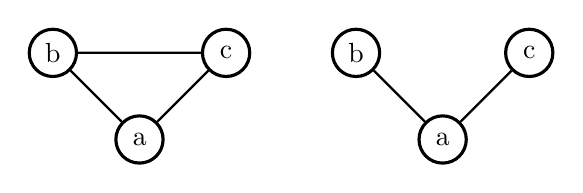
\begin{tikzpicture}[scale=1.1]

% First graph (a-b-c-a)
\node[circle, draw, minimum size=0.6cm, inner sep=0pt, line width=0.4mm] (a1) at (0, 1) {b};
\node[circle, draw, minimum size=0.6cm, inner sep=0pt, line width=0.4mm] (b1) at (2, 1) {c};
\node[circle, draw, minimum size=0.6cm, inner sep=0pt, line width=0.4mm] (c1) at (1, 0) {a};

\draw[thick] (a1) -- (b1);
\draw[thick] (b1) -- (c1);
\draw[thick] (c1) -- (a1);

% Second graph (b-a-c) with reduced space
\node[circle, draw, minimum size=0.6cm, inner sep=0pt, line width=0.4mm] (b2) at (3.5, 1) {b};
\node[circle, draw, minimum size=0.6cm, inner sep=0pt, line width=0.4mm] (a2) at (5.5, 1) {c};
\node[circle, draw, minimum size=0.6cm, inner sep=0pt, line width=0.4mm] (c2) at (4.5, 0) {a};

\draw[thick] (a2) -- (c2);
\draw[thick] (c2) -- (b2);
\end{tikzpicture}
    \end{center}
    \caption{Example of two graphs that are $2$-hop similar but not $2$-hop isomorphic. The left graph shows a complete connection between nodes $a$, $b$, and $c$, while the right graph has the same nodes connected in a path configuration.}
    \label{fig:two_hop_iso}
\end{figure}
To better understand this, consider the example in Figure \ref{fig:two_hop_iso}. Graph 1 and Graph 2 have identical 2-hop neighborhoods for their respective nodes; however, the induced subgraphs (consisting of nodes within 2 hops and the edges between them) for node ``$a$'' are not isomorphic\footnote{The left graph will induce a complete connection between nodes $a$, $b$, and $c$, while the right graph has the same nodes connected in a path configuration.}. Indeed, $k$-hop isomorphism implies $k$-hop similarity, as the latter requires only matching $k$-hop neighborhoods without enforcing identical edge connectivity within these neighborhoods.

\begin{proposition}[\textbf{Isomorphism Implies Similarity}] If two graphs are $k$-hop isomorphic, they are necessarily $k$-hop similar, but the reverse is not always true. \end{proposition}

An alternative interpretation of $k$-hop similarity is that $G_1$ and $G_2$ are considered $k$-hop similar if they can be viewed as $k$-th roots of the same graph $G$. In other terms, $G$ is the $k$-th power graph of both graphs $G1$ and $G_2$.

\begin{definition}[\textbf{$k$-th Power of a Graph}] 
The $k$-th power of a graph $G = (V, E)$, denoted $G^k$, is a graph where there is an edge between nodes $u$ and $v$ if and only if the shortest path distance between them in $G$ is at most $k$. 
\end{definition}

This leads to a practical test for $k$-hop similarity: $G_1$ and $G_2$ are $k$-hop similar if and only if their $k$-th power graphs are identical.

\begin{proposition}[\textbf{Binary $k$-Hop Reachability}]Let $\mathbf{A}_1$ and $\mathbf{A}_2$ be the adjacency matrices of $G_1$ and $G_2$, respectively. Then $G_1$ and $G_2$ are $k$-hop similar if and only if their binary $k$-hop reachability matrices satisfy:
$$R_1 = R_2,$$
where the binary $k$-hop reachability matrix $R_i$ is defined as $R_i = (A_1 + A_i^2 + \cdots + A_i^k > 0)$.
\end{proposition}

Now, the key question arises: how can we generate $k$-hop similar graphs, as we will need them to validate our hypothesis? Intuitively, one might consider computing the $k$-th power graph and then finding its roots. However, this approach is computationally challenging.

\begin{theorem}[\textbf{NP-Hardness}] Computing the roots of the $k$-th power graph is NP-hard.\end{theorem}

\subsection{Constructing $k$-Hop Similar Graphs}
Rather than directly computing the roots of the $k$-th power graph for a given input graph, we propose perturbing the original graph by removing edges, while preserving $k$-hop similarity. To achieve this, we focus on non-critical edges, which we define as edges that do not impact the $k$-hop neighborhoods of the graph.

Specifically, we aim to remove existing edges in such a way that the $k$-hop neighborhoods remain unchanged. To verify that the $k$-hop similarity is preserved, we use the distance matrix, which provides the shortest path distance between any two nodes. If two nodes are within a distance of $k$, we ensure that the operation does not increase the distance beyond $k$. Similarly, if the distance between two nodes is greater than $k$, our operation should not reduce it to less than $k$. To compute the distance matrix, we employ the Floyd-Warshall algorithm.  Algorithm \ref{alg:khopbasic} summarizes our procedure.
\begin{algorithm}[H]
\caption{Generate $K$-Hop Similar Graph}
\label{alg:khopbasic}
\begin{algorithmic}[1]
\REQUIRE{Adjacency matrix $A$, hop count $k$}
\ENSURE{A $k$-hop similar graph $G_{k}$}

\STATE $E \gets \textsc{GetEdges}(A)$
\STATE $G_{k} \gets A$ \hfill $\triangleright$ Copy of adjacency matrix
\STATE $D \gets \textsc{FloydWarshall}(G_{k})$
\STATE $paths_{k} \gets [D \leq k]$ \hfill $\triangleright$ $k$-hop paths

\FOR{each edge $(i,j)$ in $E$}
    \STATE $G_{temp} \gets G_{k}$ \hfill Temporary copy of current graph
    \STATE $G_{temp}[i,j] \gets 0$
    \STATE $G_{temp}[j,i] \gets 0$
    
    \STATE $D_{temp} \gets \textsc{FloydWarshall}(G_{temp})$
    \STATE $paths_{temp} \gets  [D_{temp} \leq k]$
    
    \IF{$paths_{temp} = paths_{k}$}
        \STATE $G_{k}[i,j] \gets 0$
        \STATE $G_{k}[j,i] \gets 0$
        \STATE $D \gets D_{temp}$
    \ENDIF
    
\ENDFOR

\STATE \textbf{return} $G_{k}$
\end{algorithmic}
\end{algorithm}

However, the complexity of this algorithm is quite high, which makes it impractical for very large graphs. The complexity arises from the need to traverse the edge set $E$ for edge removal, and for each edge traversal, compute the distance matrix using Floyd-Warshall \cite{floyd_warshall}, which has a time complexity of $O(V^3)$, where $V$ is the number of vertices. Thus, resulting in an overall complexity of $O(E \times V^3)$.

To address this high complexity, we propose the following modifications:

\begin{enumerate}
    \item \textbf{Threshold on Removals}: We introduce a threshold on the number of edges to remove. The goal is to ensure that the generated graph is structurally different from the original graph. A common measure of structural difference is the graph edit distance, which counts the minimum number of operations required to transform one graph into another. In our case, this would correspond to the number of edges we removed. We define the threshold on the graph edit distance, and once this threshold is reached, we stop exploring further edge modifications.

    \item \textbf{Batching Edge Modifications}: Instead of modifying one edge at a time, we can perform edge removals in batches. This reduces the number of edge traversals and the number of times the distance matrix needs to be recomputed. By processing multiple edges in a single step, we can significantly reduce the overall computational complexity.
\end{enumerate}

\begin{algorithm}[H]
\caption{Generate K-Hop Similar Graph with Batch Processing and Removal Thresholding}
\label{alg:improved_khop}
\begin{algorithmic}[1]
\REQUIRE{Adjacency matrix $A$, hop count $k$, removal threshold $T$, batch size $b$}
\ENSURE{A $k$-hop similar graph $G_k$}
\STATE $(E \gets \textsc{GetEdges}(A)$ \hfill $\triangleright$ Get edge and complementary lists
\STATE $G_{k} \gets A$ \hfill $\triangleright$ Copy of adjacency matrix
\STATE $D \gets \textsc{FloydWarshall}(G_{k})$
\STATE $path_{k} \gets [D\leq k]$ \hfill $\triangleright$$k$-hop paths
\STATE $removals \gets 0$
\FOR{$start \gets 0$ to $|E|$ step $b$}
    \STATE $batch \gets E[start:start+b]$ \hfill $\triangleright$Get current batch of edges
    \STATE $G_{temp} \gets G_{k}$ \hfill $\triangleright$ Temporary copy of current graph
    \FOR{each edge $(i,j)$ in $batch$}
        \STATE $G_{temp}[i,j] \gets 0$
        \STATE $G_{temp}[j,i] \gets 0$
    \ENDFOR  
    \STATE $D_{temp} \gets \textsc{FloydWarshall}(G_{temp})$
    \STATE $path_{temp} \gets [D_{temp} \leq k]$
    \IF{$path_{temp} = path_{k}$}
        \FOR{each edge $(i,j)$ in $batch$}
            \STATE $G_{k}[i,j] \gets 0$
            \STATE $G_{k}[j,i] \gets 0$
        \ENDFOR
        \STATE $D \gets D_{temp}$
        \STATE $removals \gets removals + |batch|$
    \ENDIF   
    \IF{$removals \geq T$}
        \STATE \textbf{return} $G_{k}$
    \ENDIF
\ENDFOR
\STATE \textbf{return} $G_{k}$
\end{algorithmic}
\end{algorithm}
By introducing these modifications, we aim to reduce the time complexity of Algorithm \ref{alg:khopbasic} while maintaining the core objective of perturbing the graph without violating $k$-hop similarity. The threshold on removals controls structural changes by limiting edge modifications, while batching improves efficiency by grouping operations, thus reducing the number of distance matrix computations. The resulting complexity of $O\left(\frac{T \times V^3}{b}\right)$ significantly improves efficiency for larger graphs, where $T$ is the number of edges to modify, $b$ is the batch size and $V$ is the number of nodes. Algorithm \ref{alg:improved_khop} provides a  summary of our approach for constructing $k$-hop similar graphs.

\subsection{Conjecture Validation}
In this section, we conduct a series of experiments to validate our conjecture. To evaluate it across different graph structures, we focus on node classification using synthetic datasets generated with Stochastic Block Models (SBMs) \cite{stochastic_block_models}. SBMs provide a controlled environment for analyzing the influence of structural properties and closely resemble community-structured real-world networks, making them a suitable benchmark for studying the impact of graph structure on our conjecture validity.

After training the GNNs, we validate our conjecture by measuring the level of disagreement between the learned functions trained on two $k$-hop similar graphs. By quantifying disagreement, we aim to understand the sensitivity of learned representations to local structural changes. 

In this context, we define the level of disagreement as: 
\begin{definition}[\textbf{Level of Disagreement}]
The level of disagreement measures the fraction of nodes where the predictions differ between the original graph $ G_1 $ and the $k$-hop similar graph $ G_2 $. Formally:
\[
\text{Disagreement} = \frac{1}{N} \sum_{i=1}^N \mathbb{I}(\hat{y}_i^{(1)} \neq \hat{y}_i^{(2)}),
\]
where:
\begin{itemize}
    \item $ \hat{y}_i^{(1)} $ and $ \hat{y}_i^{(2)} $ are the predicted labels for node $ i $ in $ G_1 $ and $ G_2 $, respectively,
    \item $ \mathbb{I}(\cdot) $ is the indicator function,
    \item $ N $ is the total number of nodes.
\end{itemize}
\end{definition}
\subsubsection{Synthetic Dataset Generation}
We conduct node classification experiments on synthetic graphs generated using stochastic block models (SBMs) to analyze the sensitivity of our assumptions to variations in graph structure. Our base configuration consists of $1500$ nodes, intracluster edge probability of $0.5$, intercluster edge probability of $0.1$, and $2$ classes. To isolate the influence of each parameter, we perform controlled experiments where we fix all other parameters and vary one at a time. Specifically, we vary the number of nodes between $50$ and $3000$, intra-cluster edge probability between $0.1$ and $0.9$, inter-cluster edge probability between $0.1$ and $0.9$, and the number of classes between $2$ and $10$.

Node features are sampled from a $1024$-dimensional Gaussian distribution, where each class has a unique mean vector equal to its class label, and variance is set to $1$. The dataset is approximately balanced, with an equal number of nodes per class. We use a $80/20/20$ split for training, validation, and testing, respectively
 
\subsubsection{Experimental Setting}
For $k$-hop similar graph generation, we use Algorithm \ref{alg:improved_khop} and set the graph edit distance threshold to $20\%$ of the edges in the original input graph. The batch size is chosen such that it corresponds to half of the edges to be removed. This ensures a trade-off between generating diverse graph structures while maintaining $k$-hop similarity to the original graph.

We train a two-layer Graph Convolutional Neural Network (GCN) \cite{kipf2017semisupervisedclassificationgraphconvolutional} with ReLU activation, and $32$ hidden units.

All models are trained using the Adam optimizer \cite{kingma2017adammethodstochasticoptimization}  with a learning rate of 0.01 for up to $200$ epochs. Early stopping is applied based on validation loss, using a window size of $50$ epochs. Performance is evaluated using accuracy and the level of disagreement across all datasets. 

All experimental results are averaged over $10$ independent runs with different random initializations to ensure statistical robustness, reporting both mean and standard deviation (mean $\pm$ std).


\subsubsection{Numerical Results}
\paragraph{Number of nodes.}
Table \ref{tab:number_nodes} compares the performance of the model on original and $k$-hop similar graphs with varying node counts (ranging from $50$ to $3,000$). The results strongly validate the weight consistency conjecture, showing that $ f_{\theta_1} \approx f_{\theta_2} $ holds for different graph scales. This is reflected in the exceptionally low disagreement rates ($\leq 0.69\%$) and nearly identical accuracy scores between graph pairs, despite notable structural differences ($20\%$ edges are different).
\begin{table}[H]
\caption{Performance comparison across different number of nodes. Results show classification accuracy (\%) on original and $K$-hop similar graphs, and level of disagreement (\%). All metrics are reported as mean $\pm$ standard deviation over $10$ runs.}
\label{tab:number_nodes}
\vskip 0.15in
\begin{center}
\resizebox{0.6\columnwidth}{!}{
\begin{small}
\begin{sc}
\begin{tabular}{r|ccc}
\toprule
\textbf{Nodes} & \textbf{Original Graph Acc.} & \textbf{K-Hop Graph Acc.} & \textbf{Disagreement} \\
\midrule
50 & 94.00 $\pm$ 18.00 & 94.00 $\pm$ 18.00 & 0.20 $\pm$ 0.60  \\
100 & 100.00 $\pm$ 0.00 & 100.00 $\pm$ 0.00 & 0.00 $\pm$ 0.00  \\
500 & 92.40 $\pm$ 3.35 & 92.20 $\pm$ 2.56 & 0.32 $\pm$ 0.39  \\
1000 & 98.45 $\pm$ 2.81 & 97.75 $\pm$ 3.24 & 0.69 $\pm$ 1.06 \\
1500 & 99.97 $\pm$ 0.10 & 99.97 $\pm$ 0.10 & 0.06 $\pm$ 0.18 \\
2000 & 98.65 $\pm$ 2.64 & 98.67 $\pm$ 2.65 & 0.02 $\pm$ 0.03  \\
2500 & 99.26 $\pm$ 2.22 & 99.26 $\pm$ 2.22 & 0.00 $\pm$ 0.00  \\
3000 & 100.00 $\pm$ 0.00 & 100.00 $\pm$ 0.00 & 0.00 $\pm$ 0.00  \\
\bottomrule
\end{tabular}
\end{sc}
\end{small}
}
\end{center}
\vskip -0.1in
\end{table}


\paragraph{Intracluster Probability.}

Table \ref{tab:intraclass_performance} explores the effect of varying intra-class connection probabilities (ranging from $0.2$ to $0.9$) on the consistency of the learned functions. The results strongly support $ f_{\theta_1} \approx f_{\theta_2} $, showing extremely low disagreement rates ($\leq 0.25\%$) and negligible differences in accuracy (maximum of $0.03\%$) between original and $k$-hop similar graphs. This consistency holds across all values of intraclass probability, implying that the learned functions remain largely unchanged regardless of the density of connections within the same class.
\begin{table}[H]
\caption{Performance comparison across different intraclass probability values. Results show classification accuracy (\%) on original and $K$-hop similar graphs, and level of disagreement (\%). All metrics are reported as mean $\pm$ standard deviation over $10$ runs.}
\label{tab:intraclass_performance}
\vskip 0.15in
\begin{center}
\resizebox{0.6\columnwidth}{!}{
\begin{small}
\begin{sc}
\begin{tabular}{r|ccc}
\toprule
\textbf{Intra-Class} & \textbf{Original Graph Acc.} & \textbf{K-Hop Graph Acc.} & \textbf{Disagreement} \\
\textbf{Probability} & \textbf{(\%)} & \textbf{(\%)} & \textbf{(\%)} \\
\midrule
0.2 & 88.77 $\pm$ 1.54 & 88.77 $\pm$ 1.54 & 0.00 $\pm$ 0.00 \\
0.3 & 90.80 $\pm$ 8.98 & 90.77 $\pm$ 9.07 & 0.25 $\pm$ 0.34 \\
0.4 & 99.50 $\pm$ 1.50 & 99.53 $\pm$ 1.40 & 0.03 $\pm$ 0.08 \\
0.5 & 99.40 $\pm$ 1.80 & 99.43 $\pm$ 1.70 & 0.05 $\pm$ 0.14 \\
0.6 & 97.77 $\pm$ 3.48 & 97.73 $\pm$ 3.51 & 0.02 $\pm$ 0.03 \\
0.7 & 98.97 $\pm$ 2.07 & 99.00 $\pm$ 2.01 & 0.07 $\pm$ 0.22 \\
0.8 & 100.00 $\pm$ 0.00 & 100.00 $\pm$ 0.00 & 0.00 $\pm$ 0.00 \\
0.9 & 100.00 $\pm$ 0.00 & 100.00 $\pm$ 0.00 & 0.00 $\pm$ 0.00 \\
\bottomrule
\end{tabular}
\end{sc}
\end{small}
}
\end{center}
\vskip -0.1in
\end{table}


\paragraph{Intercluster Probability.}
Table \ref{tab:interclass_performance} investigates the impact of varying interclass connection probabilities (from $0$ to $0.9$) on function consistency. Although the overall accuracy decreases with higher interclass connectivity, the approximation $ f_{\theta_1} \approx f_{\theta_2} $ remains strong, as evidenced by low disagreement rates ($\leq 0.51\%$) and consistent accuracy scores (maximum difference of $0.32\%$). This suggests that the weight consistency conjecture continues to hold even as the graph structure becomes more complex with increased interclass connectivity.
\begin{table}[H]
\caption{Performance comparison across different interclass probability values. Results show classification accuracy (\%) on original and $K$-hop similar graphs, and level of disagreement (\%). All metrics are reported as mean $\pm$ standard deviation over $10$ runs.}
\label{tab:interclass_performance}
\vskip 0.15in
\begin{center}
\resizebox{0.6\columnwidth}{!}{
\begin{small}
\begin{sc}
\begin{tabular}{r|ccc}
\toprule
\textbf{Inter-Class} & \textbf{Original Graph Acc.} & \textbf{K-Hop Graph Acc.} & \textbf{Disagreement} \\
\textbf{Probability} & \textbf{(\%)} & \textbf{(\%)} & \textbf{(\%)} \\
\midrule
0.0 & 100.00 $\pm$ 0.00 & 100.00 $\pm$ 0.00 & 0.00 $\pm$ 0.00 \\
0.1 & 99.60 $\pm$ 1.60 & 99.92 $\pm$ 0.30 & 0.28 $\pm$ 1.12 \\
0.2 & 99.73 $\pm$ 1.32 & 99.94 $\pm$ 0.24 & 0.20 $\pm$ 0.92 \\
0.3 & 92.57 $\pm$ 13.23 & 92.47 $\pm$ 13.67 & 0.51 $\pm$ 1.22 \\
0.4 & 86.91 $\pm$ 16.47 & 86.83 $\pm$ 16.73 & 0.41 $\pm$ 1.11 \\
0.5 & 83.68 $\pm$ 16.70 & 83.61 $\pm$ 16.90 & 0.34 $\pm$ 1.02 \\
0.6 & 80.72 $\pm$ 17.11 & 80.66 $\pm$ 17.27 & 0.30 $\pm$ 0.96 \\
0.7 & 78.55 $\pm$ 17.04 & 78.49 $\pm$ 17.17 & 0.26 $\pm$ 0.90 \\
0.8 & 76.87 $\pm$ 16.78 & 76.83 $\pm$ 16.89 & 0.23 $\pm$ 0.85 \\
0.9 & 75.66 $\pm$ 16.35 & 75.62 $\pm$ 16.46 & 0.21 $\pm$ 0.81 \\
\bottomrule
\end{tabular}
\end{sc}
\end{small}
}
\end{center}
\end{table}

\paragraph{Number of classes.}
Table \ref{tab:classes_performance} reveals a surprising behavior when examining the weight consistency conjecture across different numbers of classes (ranging from $2$ to $10$). While \( f_{\theta_1} \approx f_{\theta_2} \) holds strongly for binary and three-class problems (with disagreement \(\leq 4.24\%\)), we observe an unexpected sharp increase in disagreement rates for higher numbers of classes, reaching up to $81.08\%$ for $10$ classes. Intriguingly, despite this high disagreement in individual predictions, both models maintain remarkably similar overall accuracy scores (with a maximum difference of $2.47\%$).
\begin{table}[H]
\caption{Performance comparison across different numbers of classes. Results show classification accuracy (\%) on original and $K$-hop similar graphs, and level of disagreement (\%). All metrics are reported as mean $\pm$ standard deviation over $10$ runs.}
\label{tab:classes_performance}
\vskip 0.15in
\begin{center}
\resizebox{0.6\columnwidth}{!}{
\begin{small}
\begin{sc}
\begin{tabular}{r|ccc}
\toprule
\textbf{Number of} & \textbf{Original Graph Acc.} & \textbf{K-Hop Graph Acc.} & \textbf{Disagreement} \\
\textbf{Classes} & \textbf{(\%)} & \textbf{(\%)} & \textbf{(\%)} \\
\midrule
2 & 99.43 $\pm$ 0.86 & 99.00 $\pm$ 1.48 & 0.63 $\pm$ 1.05 \\
3 & 78.27 $\pm$ 7.83 & 77.30 $\pm$ 6.54 & 4.24 $\pm$ 4.54 \\
4 & 72.20 $\pm$ 6.07 & 70.10 $\pm$ 3.49 & 4.30 $\pm$ 4.83 \\
5 & 44.10 $\pm$ 6.05 & 46.57 $\pm$ 9.35 & 45.95 $\pm$ 33.28 \\
6 & 28.87 $\pm$ 8.25 & 28.67 $\pm$ 7.70 & 73.81 $\pm$ 30.42 \\
7 & 29.37 $\pm$ 7.82 & 29.83 $\pm$ 8.11 & 54.43 $\pm$ 35.84 \\
8 & 19.63 $\pm$ 5.01 & 20.30 $\pm$ 4.90 & 78.47 $\pm$ 16.74 \\
9 & 21.17 $\pm$ 2.71 & 21.23 $\pm$ 3.89 & 77.79 $\pm$ 6.88 \\
10 & 17.33 $\pm$ 4.67 & 17.60 $\pm$ 4.82 & 81.08 $\pm$ 20.75 \\
\bottomrule
\end{tabular}
\end{sc}
\end{small}
}
\end{center}
\end{table}
Investigating the predicted class probabilities reveals that this apparent contradiction arises from model uncertainty. As the number of classes increases, the models produce increasingly uniform probability distributions across classes, indicating low confidence in their predictions. This explains why small perturbations in input graphs can lead to different class assignments while maintaining similar accuracy levels: essentially, the models are making near-random choices among equally uncertain options. In other words, while the models may assign different classes due to subtle changes in the input, the lack of clear discrimination between classes results in similar accuracy outcomes. 

\begin{figure}[H]
    \vskip 0.2in
    \begin{center}    \centerline{\includegraphics[width=0.6\columnwidth]{Figures/mean_probs_origin.png}}
    \caption{Average predicted probability distribution across ten classes for a GNN model trained on the original graph.}
    \label{origin}
    \end{center}
    \vskip -0.2in
\end{figure}

\begin{figure}[H]
    \vskip 0.2in
    \begin{center}
    \centerline{\includegraphics[width=0.6\columnwidth]{Figures/mean_probs_origin.png}}
    \caption{Average predicted probability distribution across ten classes for a GNN model trained on the $2$-hop similar graph.}
    \label{hophop}
    \end{center}
    \vskip -0.2in
\end{figure}

Figures \ref{origin} and \ref{hophop} present the average predicted probability distribution for disagreed nodes across ten classes, comparing the models trained on the original graph and the two-hop similar graph. The near-uniform distribution (with probabilities ranging from approximately 0.08 to 0.10) indicates the model's low confidence in class assignments. Each class receives similar probability mass, regardless of the true label, which suggests that the model is uncertain in distinguishing between the classes.

This behavior suggests that the issue is not with the weight consistency conjecture itself, but rather with the model's fundamental inability to learn discriminative features for multi-class classification tasks. 


Based on our experimental analysis, we consider that Conjecture \ref{conjecture: weight_consistency} is \textbf{valid}.



\begin{table}[t]
    % \vspace{-2mm}
    \caption{Accuracy on Spurious-Motif dataset. The $\textbf{Bold}^\dagger$, $\textbf{Bold}$, and $\underline{\text{Underline}}$ highlight the first, second, and third best results, respectively. All results are reported with mean $\pm$ std.
    }
    % \vspace{-3mm}
    \centering
    \label{tab:oversmooth-spmotif}
    \resizebox{0.8\textwidth}{!}{%
        \begin{tabular}{llcccc}
            \toprule
            Dataset & Model
            & $L=3$ & $L=6$  & $L=8$ & $L=16$   \\
            \midrule
            \multirow{3}*{SPMotif-0.33} &GCN                                                   &
            $58.51 \pm 2.843$                                      & $ 60.81 \pm 5.39$                 & $64.17 \pm 3.84$ & 	$61.51 \pm 3.85$

            \\
            &+CIGA                                             &
            $67.53 \pm 1.35$                                       & $ 67.78 \pm 1.27$                  & $71.34 \pm 9.96 $ & $77.19 \pm 5.55$
            \\
            &+\ours                                            &
            $67.81 \pm 3.33 $                                       & $69.06 \pm 5.58$                  & $45.84 \pm 3.82$  & $84.31 \pm 4.65$
            \\
             \midrule
             \multirow{3}*{SPMotif-0.60} &GCN                                                   &

            $50.51 \pm 4.75$                                      & $61.20 \pm 3.11$                 & $64.55 \pm 6.02$ & $67.09 \pm 2.48$

            \\
            &+CIGA                                             &
            $59.96 \pm 8.59$                                       & $66.54 \pm 1.92$                  & $69.07 \pm 3.45 $  &$77.47 \pm 9.33$
            \\
            &+\ours                                            &
            $62.79 \pm 3.86$                                       & $ 74.21\pm 10.77$                  & $45.84 \pm 3.82$  & $85.99 \pm 2.52$ 
            \\
             \midrule
             
            \multirow{3}*{SPMotif-0.90} &GCN 
            & $44.67 \pm 5.07$                                & $63.07 \pm 3.50$                                   & $63.55\pm 6.64$ &  $ 59.08 \pm 5.87 $	\\
            &+CIGA                                             & $\textbf{47.66}\pm6.08$
            &$68.49 \pm 0.99$                                       & $74.67	\pm 10.62$  & $76.93	\pm 12.49$\\
            &+\ours                                         & $\textbf{50.93}^\dagger\pm9.05$
            &$\underline{81.64} \pm 8.37$                                       & $74.67	\pm 10.62$ &  $87.05 \pm 3.36$\\
            \bottomrule
           
        \end{tabular}%
    }
    %\vspace{-4.4mm}
\end{table}
\section*{Conclusion}
This paper aims to enhance our understanding of the computational complexity of computing various Shapley value variants. We found that for various ML models --- including decision trees, regression tree ensembles, weighted automata, and linear regression --- both local and global interventional and baseline SHAP can be computed in polynomial time under HMM modeled distributions. This extends popular algorithms, such as TreeSHAP, beyond their empirical distributional scope. We also establish strict complexity gaps between the various SHAP variants (baseline, interventional, and conditional) and prove the intractability of computing SHAP for tree ensembles and neural networks in simplified scenarios. Overall, we present SHAP as a versatile framework whose complexity depends on four key factors: \begin{inparaenum}[(i)] \item model type, \item SHAP variant, \item distribution modeling approach, \item and local vs. global explanations\end{inparaenum}. We believe this perspective provides deeper insight into the computational complexity of SHAP, paving the way for future work.




%We believe that our framework provides a more intricate understanding of SHAP computation complexity across different models, distributions, and variants, paving the way for further research.

Our work opens promising directions for future research. First, expanding our computational analysis to other SHAP-related metrics, such as asymmetric SHAP~\citep{frye20} and SAGE~\citep{covert2020understanding}, would be valuable. Additionally, we aim to explore more expressive distribution classes and relaxed assumptions beyond those in Section \ref{sec:tractable} while maintaining tractable SHAP computation. Finally, when exact computation is intractable (Section \ref{sec:intractable}), investigating the approximability of SHAP metrics through approximation and parameterized complexity theory~\citep{downey2012parameterized} is an important direction.

%Our work opens several promising avenues for future research on the computational properties of explainable AI methods, with a particular focus on SHAP. First, it would be interesting to broaden the computational analysis conducted in this work to include other popular SHAP-related metrics in the literature, such as asymmetric SHAP \cite{frye20} and SAGE \cite{covert2020understanding}. Also, in the future, we aim to explore more expressive distribution classes and relaxed distributional assumptions—extending beyond those examined in Section \ref{sec:tractable} —that still yield tractable SHAP computation. Finally, when exact computation proves intractable (Section \ref{sec:intractable}), it is worthwhile to theoretically investigate the question of the approximability of computing the SHAP metrics across various configurations, through the lens of approximation and parametrized complexity theory \cite{arora2009computational}.

%This paper aims to deepen our understanding of the computational complexity involved in obtaining different Shapley value variants. We found that for a variety of ML models, including decision trees, tree ensembles for regression, weighted automata, and linear regression models — computing both local and global interventional and baseline SHAP can be done in polynomial time when distributions are modeled by HMMs. This extends the distributional scope of popular algorithms like TreeSHAP, which is limited to empirical distributions. Additionally, we demonstrate a strict complexity gap between SHAP variants, showing that interventional and baseline SHAP can be strictly easier to compute than conditional SHAP. Despite these positive results, we uncovered intractability for various SHAP variants in neural networks and tree ensembles. Finally, we provided generalized complexity relations across SHAP variants. We believe that our framework offers a deeper understanding of the complexity involved in computing SHAP across various variants, models, distributions, as well as in both local and global computations, laying the groundwork for future research.




\bibliographystyle{unsrtnat}
\bibliography{references} 

\end{document}
